% !TEX program = xelatex
% 高级时间序列分析 — 课程作业汇报
% 编译: xelatex beamer_presentation.tex (两次以获得目录)
\documentclass[10pt,aspectratio=169]{beamer}
\usepackage{fontspec}
\usepackage{xeCJK}
\setCJKmainfont{SimSun}
\setCJKsansfont{SimHei}
\setCJKmonofont{KaiTi}
\usepackage{graphicx}
\usepackage{booktabs}
\usepackage{amsmath}

% Beamer theme
\usetheme{Madrid}
\usecolortheme{default}
\setbeamertemplate{navigation symbols}{}

% Title
\title{中国股票市场波动聚集与风险预警：\\基于沪深300指数收益率的GARCH模型分析}
\author{汇报人：赖景祺}
\date{2026年5月}

\begin{document}

% === Slide 1: 封面 ===
\begin{frame}
  \titlepage
\end{frame}

% === Slide 2: 研究动机 ===
\begin{frame}{研究动机}
  \begin{itemize}
    \item 中国A股市场波动剧烈，风险监测是投资者与监管层的核心关切
    \item 金融风险不仅体现为价格方向变化，也体现为\textbf{不确定性程度}的时变性
    \item 大量实证研究表明金融收益率存在\textbf{波动聚集}（volatility clustering）：\\
    大波动倾向于集中出现，平静期与剧烈波动期交替
    \item 沪深300指数覆盖两市市值最大、流动性最好的300只股票，\\
    是中国A股市场最具代表性的基准指数
    \item 本文使用\textbf{GARCH族模型}研究其时变风险特征
  \end{itemize}
\end{frame}

% === Slide 3: 研究问题 ===
\begin{frame}{研究问题}
  \begin{block}{核心问题}
    \begin{enumerate}
      \item 沪深300指数日收益率是否存在\textbf{波动聚集}？
      \item GARCH模型能否\textbf{刻画其时变条件波动率}？
    \end{enumerate}
  \end{block}
  \vspace{1em}
  \textbf{重要区分：}
  \begin{itemize}
    \item GARCH刻画的是\textbf{时变条件方差}（不确定性程度）
    \item GARCH\textbf{不}预测指数涨跌方向
  \end{itemize}
\end{frame}

% === Slide 4: 数据说明 ===
\begin{frame}{数据说明}
  \begin{itemize}
    \item \textbf{数据来源：}东方财富（通过AkShare获取）
    \item \textbf{样本区间：}2002年1月7日 -- 2026年5月11日
    \item \textbf{频率：}日度
    \item \textbf{样本量：}5902个交易日
    \item \textbf{变量：}沪深300收盘价 $P_t$
    \item \textbf{数据接口：}优先 \texttt{index\_zh\_a\_hist}，回退 \texttt{stock\_zh\_index\_daily}
  \end{itemize}
\end{frame}

% === Slide 5: 收益率公式 ===
\begin{frame}{收益率计算}
  \begin{block}{百分比日对数收益率}
    \[
    r_t = 100\left[\log(P_t) - \log(P_{t-1})\right]
    \]
  \end{block}
  \begin{itemize}
    \item 对数收益率具有时间可加性
    \item 乘以100使数值以百分比为单位
    \item 删除首个缺失值后得到5902个有效观测
  \end{itemize}
\end{frame}

% === Slide 6: 描述性统计表 ===
\begin{frame}{描述性统计}
  \begin{table}
    \centering
    \begin{tabular}{lr}
      \toprule
      统计量 & 数值 \\
      \midrule
      样本量 & 5902 \\
      均值 (\%) & 0.0224 \\
      标准差 (\%) & 1.5572 \\
      最小值 (\%) & --9.6949 \\
      最大值 (\%) & 8.9743 \\
      偏度 & --0.3820 \\
      超额峰度 & 4.7273 \\
      \bottomrule
    \end{tabular}
  \end{table}
  \begin{itemize}
    \item 均值接近零，标准差约1.56\%
    \item 偏度为负（左偏），峰度远大于0：\textbf{尖峰厚尾}
  \end{itemize}
\end{frame}

% === Slide 7: 收益率图 ===
\begin{frame}{收益率与平方收益率}
  \begin{center}
    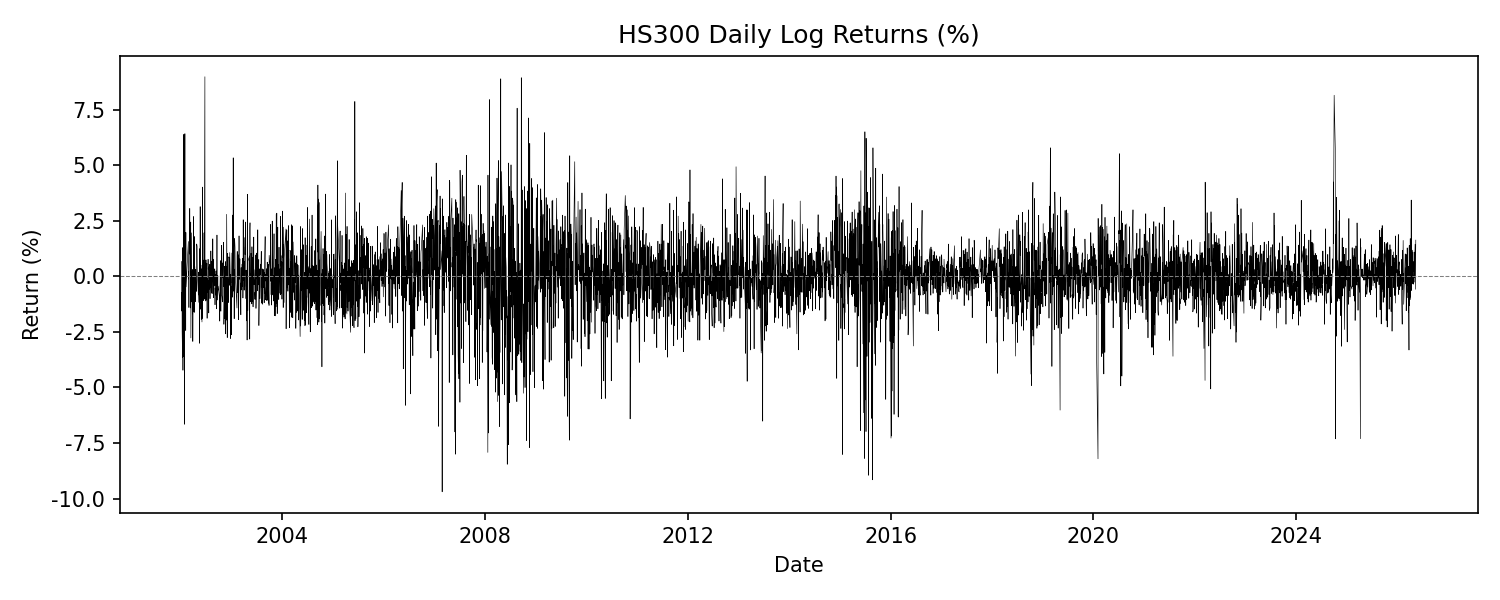
\includegraphics[width=0.95\textwidth,height=0.35\textheight,keepaspectratio]{../figures/fig2_hs300_returns.png}\\[0.5em]
    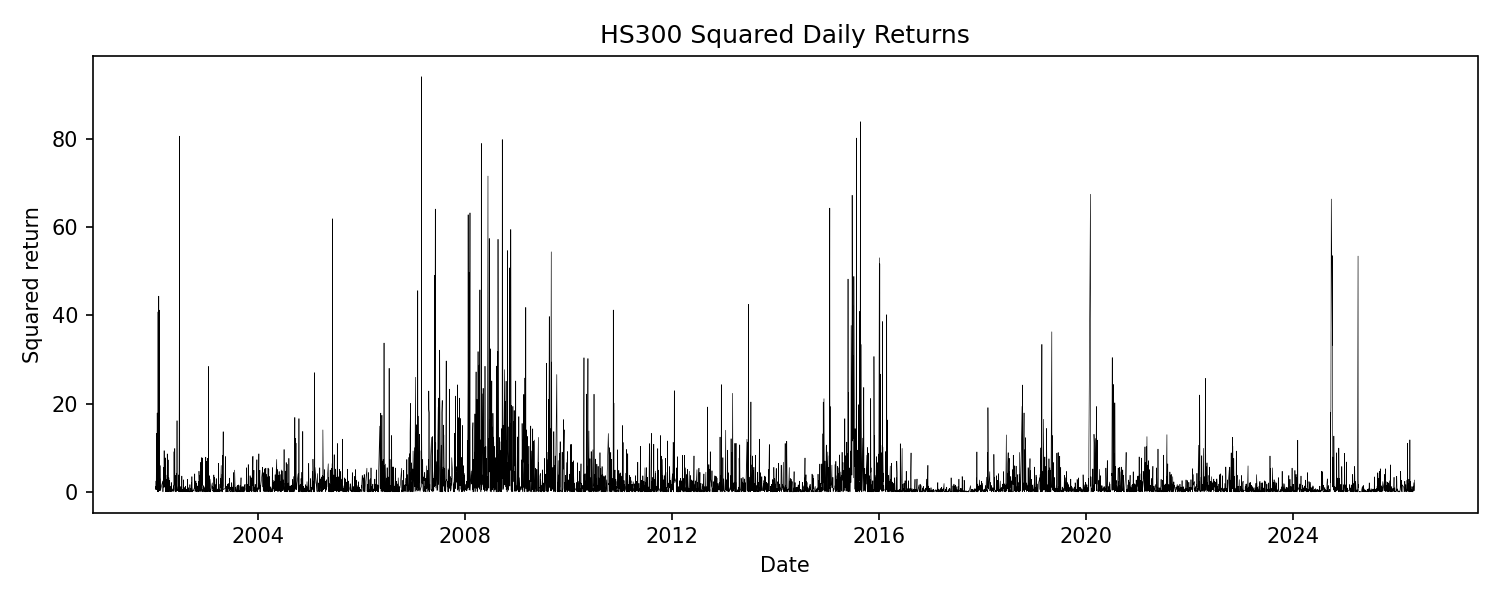
\includegraphics[width=0.95\textwidth,height=0.35\textheight,keepaspectratio]{../figures/fig3_hs300_squared_returns.png}
  \end{center}
  \begin{itemize}
    \item 波动在2008、2015、2020年剧烈放大——\textbf{波动聚集}
  \end{itemize}
\end{frame}

% === Slide 8: 分布直方图 ===
\begin{frame}{收益率分布}
  \begin{center}
    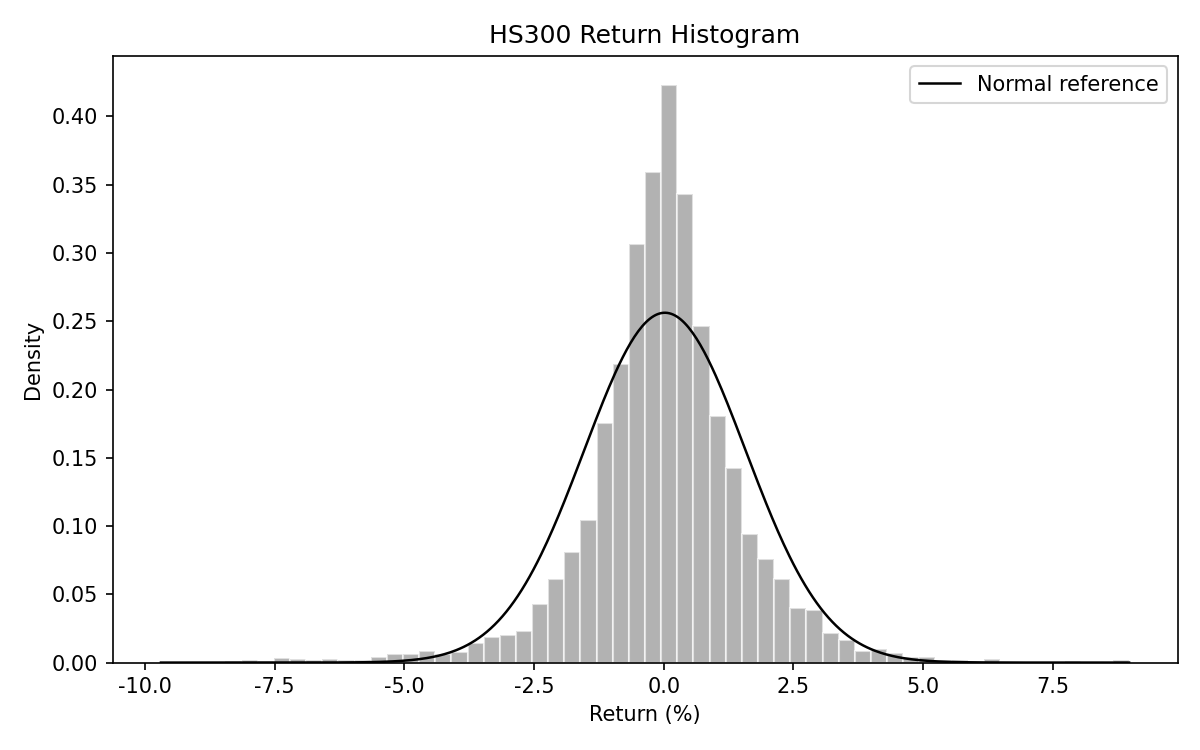
\includegraphics[width=0.7\textwidth,height=0.5\textheight,keepaspectratio]{../figures/fig4_return_histogram.png}
  \end{center}
  \begin{itemize}
    \item 实际分布比正态更尖、尾更厚\\
    \item 极端值频次远高于正态预期
  \end{itemize}
\end{frame}

% === Slide 9: 方法论 — GARCH(1,1) ===
\begin{frame}{方法：GARCH(1,1)模型}
  \begin{block}{均值方程}
    \[ r_t = \mu + \varepsilon_t \]
  \end{block}
  \begin{block}{方差方程}
    \[ \varepsilon_t = \sigma_t z_t, \quad z_t \stackrel{i.i.d.}{\sim} N(0,1) \]
    \[ \sigma_t^2 = \omega + \alpha \varepsilon_{t-1}^2 + \beta \sigma_{t-1}^2 \]
  \end{block}
  \begin{itemize}
    \item $\omega$：基础波动水平；$\alpha$：新冲击效应（ARCH）
    \item $\beta$：波动持续性（GARCH）；$\alpha+\beta$：持久性指数
    \item $\alpha+\beta<1$：弱平稳；$\alpha+\beta=1$：IGARCH边界
    \item 半衰期：$\log(0.5)/\log(\alpha+\beta)$
  \end{itemize}
\end{frame}

% === Slide 10: 预备检验 ===
\begin{frame}{预备检验}
  \begin{table}
    \centering
    \begin{tabular}{lrrl}
      \toprule
      检验 & 滞后 & 统计量 & 结果 \\
      \midrule
      ADF & 14 & --18.10 & 平稳 $(p\approx 0)$ \\
      Ljung-Box($r_t^2$) & 10 & 1525.78 & 波动聚集 $(p\approx 0)$ \\
      Ljung-Box($r_t^2$) & 20 & 2379.28 & 波动聚集 $(p\approx 0)$ \\
      ARCH-LM & 5 & 529.63 & ARCH效应 $(p\approx 0)$ \\
      ARCH-LM & 10 & 634.52 & ARCH效应 $(p\approx 0)$ \\
      ARCH-LM & 12 & 636.83 & ARCH效应 $(p\approx 0)$ \\
      \bottomrule
    \end{tabular}
  \end{table}
  \begin{itemize}
    \item 收益率平稳 $\checkmark$；强烈的波动聚集证据 $\checkmark$\\
    \item 使用GARCH具有充分的统计依据
  \end{itemize}
\end{frame}

% === Slide 11: GARCH(1,1)主结果 ===
\begin{frame}{GARCH(1,1)参数估计}
  \begin{table}
    \centering
    \begin{tabular}{lrrrl}
      \toprule
      参数 & 估计值 & 标准误 & t值 & p值 \\
      \midrule
      $\mu$ & 0.0247 & 0.0159 & 1.546 & 0.122 \\
      $\omega$ & 0.0216 & 0.0066 & 3.281 & 0.001 \\
      $\alpha$ & 0.0734 & 0.0103 & 7.113 & $<0.001$ \\
      $\beta$ & 0.9195 & 0.0104 & 88.239 & $<0.001$ \\
      \midrule
      $\alpha+\beta$ & \multicolumn{4}{c}{0.9928} \\
      半衰期 & \multicolumn{4}{c}{96.3 个交易日（约4.6个月）} \\
      AIC / BIC & \multicolumn{4}{c}{20313.98 / 20340.71} \\
      \bottomrule
    \end{tabular}
  \end{table}
  \begin{itemize}
    \item $\alpha$显著$>0$：新冲击抬升未来波动
    \item $\beta$极大：波动一旦升高将持续较长时间
    \item $\alpha+\beta\approx1$：近IGARCH，波动极为持久
  \end{itemize}
\end{frame}

% === Slide 12: 条件波动率 ===
\begin{frame}{条件波动率估计}
  \begin{center}
    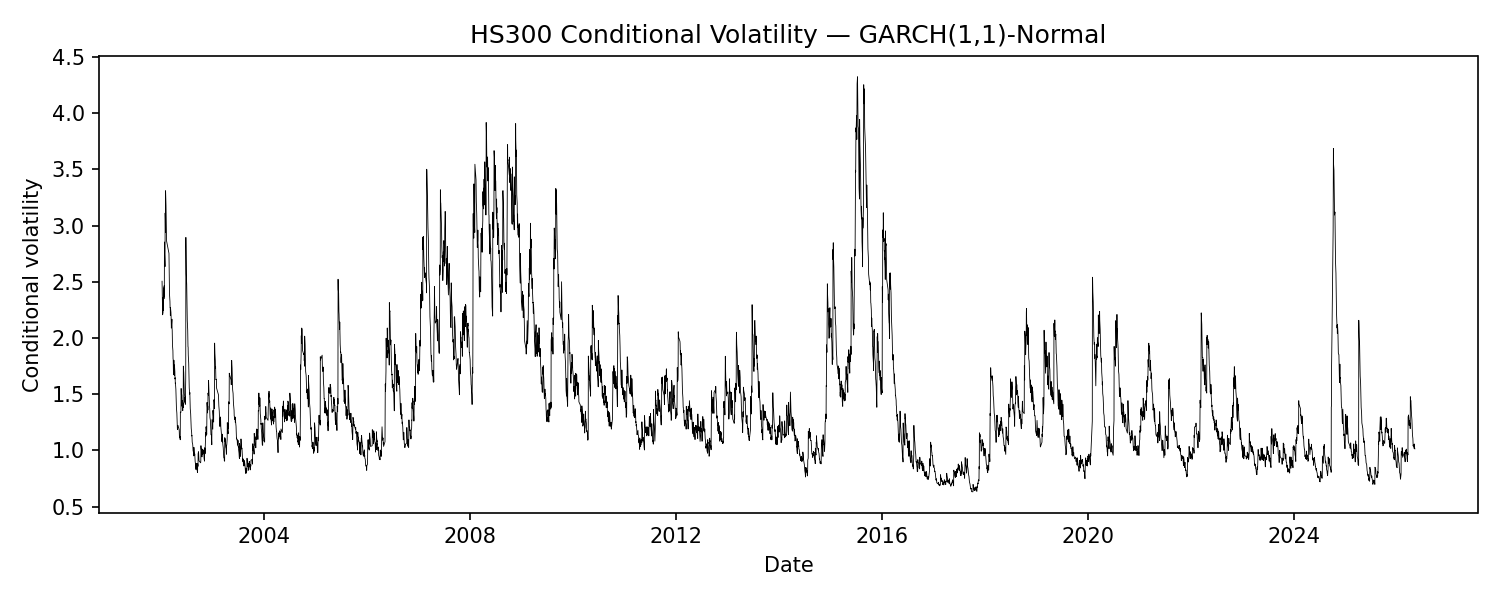
\includegraphics[width=0.95\textwidth,height=0.55\textheight,keepaspectratio]{../figures/fig5_garch_conditional_volatility.png}
  \end{center}
  \begin{itemize}
    \item 模型识别出2008、2015、2020年高风险时段
    \item 条件波动率反映\textbf{时变风险状态}，不是涨跌方向
  \end{itemize}
\end{frame}

% === Slide 13: 残差诊断 ===
\begin{frame}{残差诊断}
  \begin{table}
    \centering
    \begin{tabular}{lrrl}
      \toprule
      检验 & 统计量 & p值 & 结论 \\
      \midrule
      LB($z_t$) lag=10 & 40.48 & 0.000 & 仍有自相关 \\
      LB($z_t$) lag=20 & 48.42 & 0.000 & 仍有自相关 \\
      LB($z_t^2$) lag=10 & 4.39 & 0.928 & 异方差已被捕捉 \\
      LB($z_t^2$) lag=20 & 9.66 & 0.974 & 异方差已被捕捉 \\
      ARCH-LM($z_t$) lag=5 & 2.29 & 0.808 & 无异方差残留 \\
      \bottomrule
    \end{tabular}
  \end{table}
  \begin{itemize}
    \item \textbf{$z_t^2$ 和 ARCH-LM干净} $\Rightarrow$ GARCH捕捉了主要条件异方差
    \item $z_t$仍有自相关 $\Rightarrow$ 常数均值方程可以改进
  \end{itemize}
\end{frame}

% === Slide 14: 稳健性 — Student-t ===
\begin{frame}{稳健性1: Student-t GARCH(1,1)}
  \begin{columns}
    \column{0.5\textwidth}
      \begin{itemize}
        \item 创新分布：$z_t \sim t(\nu)$
        \item $\hat{\nu}=5.1541$：尾部显著厚于正态
      \end{itemize}
    \column{0.5\textwidth}
      \begin{table}
        \centering
        \begin{tabular}{lrr}
          \toprule
          & Normal & Student-t \\
          \midrule
          AIC & 20314 & \textbf{19902} \\
          BIC & 20341 & \textbf{19935} \\
          $\alpha+\beta$ & 0.9928 & 0.9946 \\
          \bottomrule
        \end{tabular}
      \end{table}
  \end{columns}
  \vspace{1em}
  \begin{block}{结论}
    Student-t显著优于正态（AIC低412），\textbf{收益率厚尾特征得到确认}。\\
    核心结论（波动聚集、高持久性）不依赖正态分布假设。
  \end{block}
\end{frame}

% === Slide 15: 稳健性 — GJR-GARCH ===
\begin{frame}{稳健性2: GJR-GARCH(1,1) — Normal vs Student-t}
  \begin{block}{GJR-GARCH方差方程}
    \[
    \sigma_t^2 = \omega + \alpha \varepsilon_{t-1}^2 + \gamma\,I(\varepsilon_{t-1}<0)\,\varepsilon_{t-1}^2 + \beta \sigma_{t-1}^2
    \]
  \end{block}
  \begin{table}
    \centering
    \begin{tabular}{lccc}
      \toprule
      & GJR-Normal & GJR-Student-t \\
      \midrule
      $\gamma$ & 0.0159 & 0.0217 \\
      p($\gamma$) & 0.217 & \textbf{0.046} \\
      AIC & 20312 & \textbf{19899} \\
      $\nu$ & -- & 5.14 \\
      \bottomrule
    \end{tabular}
  \end{table}
  \begin{itemize}
    \item 正态假设下$\gamma$不显著；\textbf{厚尾Student-t下$\gamma$达5\%显著}
    \item 分布误设可能掩盖非对称效应；厚尾分布对识别非对称至关重要
  \end{itemize}
\end{frame}

% === Slide 16: 稳健性 — EGARCH ===
\begin{frame}{稳健性3: EGARCH(1,1)}
  \begin{block}{EGARCH方差方程（对数形式）}
    \[
    \ln\sigma_t^2 = \omega + \alpha(|z_{t-1}|-\mathbb{E}|z_{t-1}|) + \gamma z_{t-1} + \beta\ln\sigma_{t-1}^2
    \]
  \end{block}
  \begin{itemize}
    \item $\alpha$：冲击幅度效应；$\gamma$：符号/非对称效应；$\beta$：对数方差持续性
    \item $\gamma<0$表示负向冲击提高未来对数条件方差（杠杆效应方向）
  \end{itemize}
  \begin{table}
    \centering
    \begin{tabular}{lcc}
      \toprule
      & EGARCH-Normal & EGARCH-Student-t \\
      \midrule
      $\gamma$ & $-0.0121$ & $-0.0123$ \\
      p($\gamma$) & 0.213 & 0.101 \\
      AIC & 20299 & \textbf{19876} \\
      $\nu$ & -- & 5.19 \\
      \bottomrule
    \end{tabular}
  \end{table}
  \begin{block}{结论}
    EGARCH非对称项均未达5\%显著；Student-t下p=0.101，\\
    接近10\%边界但未达常用显著性水平——\textbf{非对称证据对模型形式敏感}。
  \end{block}
\end{frame}

% === Slide 17: 稳健性 — AR(1)-GARCH ===
\begin{frame}{稳健性4: AR(1)-GARCH(1,1)}
  \begin{block}{均值方程}
    \[ r_t = \phi_0 + \phi_1 r_{t-1} + \varepsilon_t \]
  \end{block}
  \begin{itemize}
    \item 方差方程保持GARCH(1,1)不变
    \item $\hat{\phi}_1=0.0240$，AIC=20308.85（常数均值GARCH: 20313.98）
    \item AIC略低约5点：均值方程存在改进空间但影响有限
    \item $\alpha+\beta=0.9928$与主模型几乎一致
  \end{itemize}
  \begin{block}{结论}
    均值方程的微小调整对波动持续性结论\textbf{影响不显著}，\\
    主要结论保持稳健。
  \end{block}
\end{frame}

% === Slide 18: 核心发现 ===
\begin{frame}{核心发现}
  \begin{enumerate}
    \item \textbf{波动聚集存在}\\
    沪深300日收益率存在显著的波动聚集；\\
    ARCH-LM强烈拒绝无ARCH效应原假设

    \item \textbf{GARCH(1,1)有效}\\
    $\alpha=0.0734$ $(p<0.001)$，$\beta=0.9195$ $(p<0.001)$；\\
    模型较好捕捉了条件异方差结构

    \item \textbf{波动高度持久}\\
    $\alpha+\beta=0.9928$，半衰期$\approx$96个交易日

    \item \textbf{厚尾特征稳健确认}\\
    Student-t分布在所有模型设定中均远优于正态（AIC降幅$>$400）

    \item \textbf{非对称效应：部分证据，模型敏感}\\
    GJR-Student-t: $\gamma=0.0217$，$p=0.046$（5\%显著）\\
    EGARCH-Student-t: $\gamma=-0.0123$，$p=0.101$（未达常用显著水平）
  \end{enumerate}
\end{frame}

% === Slide 19: 局限 ===
\begin{frame}{局限与证据边界}
  \begin{itemize}
    \item \textbf{GARCH是reduced-form模型}\\
    刻画条件方差的统计特征，不是结构因果模型
    \item \textbf{不预测涨跌方向}\\
    条件波动率高 $\neq$ 指数下跌，$\neq$ 指数上涨\\
    仅模型推断的不确定性程度较高
    \item \textbf{可能的结构突变}\\
    股权分置改革、融资融券、熔断机制等制度变革\\
    未被显式建模
    \item \textbf{遗漏变量}\\
    未纳入货币政策、流动性、国际市场等外部因素
    \item \textbf{非对称效应：GJR-t显著但EGARCH证据较弱}\\
    非对称结论对模型形式（GJR vs EGARCH）敏感，\\
    不能简单断言杠杆效应存在或不存在
  \end{itemize}
\end{frame}

% === Slide 20: 结论 ===
\begin{frame}{结论}
  \begin{enumerate}
    \item 沪深300日收益率存在显著的\textbf{波动聚集}，\\
    ARCH-LM检验提供了明确统计证据
    \item GARCH(1,1)能够刻画\textbf{时变条件波动率}，\\
    波动冲击高度持久（$\alpha+\beta=0.9928$）
    \item \textbf{厚尾分布稳健重要}：Student-t在所有模型设定中远优于正态
    \item \textbf{非对称效应部分支持}：GJR-Student-t下$\gamma$显著（$p=0.046$），\\
    但EGARCH证据较弱（$p=0.101$），结论对模型形式敏感
  \end{enumerate}
  \vspace{1em}
  \begin{center}
    \textbf{GARCH是风险状态建模工具，不是涨跌预测模型。}\\
    条件波动率为风险监测提供统计参考，\\
    不能替代政策判断和基本面分析。
  \end{center}
\end{frame}

% === Slide 20: 谢谢 ===
\begin{frame}
  \begin{center}
    \Huge 谢谢\\[1em]
    \Large 欢迎提问
  \end{center}
\end{frame}

\end{document}
